% Adapted from LaTeX-examples-master/tikz/triangle-menelaos-1.
\documentclass[border=2pt]{standalone}
\usepackage{tikz}
\usepackage{tkz-euclide}
\usepackage{helvet}
\usepackage[eulergreek]{sansmath}
\begin{document}
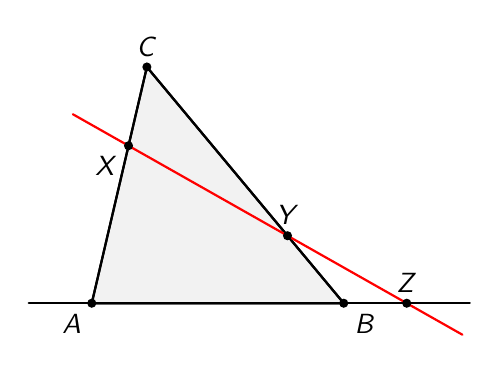
\begin{tikzpicture}[very thick,font=\sansmath\sffamily]
  \tkzDefPoint(0,0){A}
  \tkzDefPoint(3.2,0){B}
  \tkzDefPoint(4.0,0){Z}
  \tkzDefPoint(0.7,3){C}
  \tkzDefBarycentricPoint(A=1,C=2)\tkzGetPoint{X}
  \tkzInterLL(B,C)(X,Z)\tkzGetPoint{Y}

  \tkzLabelPoints[below left,font=\sansmath\sffamily](A)
  \tkzLabelPoints[below right,font=\sansmath\sffamily](B)
  \tkzLabelPoints[above,font=\sansmath\sffamily](C)
  \tkzLabelPoints[below left,font=\sansmath\sffamily](X)
  \tkzLabelPoints[above,font=\sansmath\sffamily](Z)
  \tkzLabelPoints[above,font=\sansmath\sffamily](Y)

  \tkzDrawPolygon[thick,fill=gray!10](A,B,C)
  \tkzDrawPolygon[thick](A,B,C)
  \tkzDrawLines[thick](A,Z)
  \tkzDrawLines[thick,color=red](Z,X)
  \tkzDrawPoints[color=black,shape=circle,fill=black,size=2](A,B,C,X,Y,Z)
\end{tikzpicture}
\end{document}
